
%%%
% [chapter] Förord
%
\jhchapter{Förord}

Historien kan inte tyglas, tiden visar ingen hänsyn. Det som har varit är borta och vi kan på sin höjd ana hur fenomenen i all hast dragit förbi. De minnen vi fångat är skärvor från en gemensam bakgrund som kan återges på många olika sätt. Vi har valt att berätta byhistorien med START I NUTID och därifrån steg för steg sökt oss bakåt i varje enskild lägenhets tidslinje. I huvudsak har vi valt att beskriva de senaste 200 åren, men i enskilda fall betydligt längre bakåt än så. Vi har delvis använt boken Överjeppo 2 som modell. Uppgiften har varit dryg, den har fordrat timmar och åter timmar av detekterande, gårdsbesök, intervjuer, bild- och kartstudier och rotande i många arkiv. Där det personliga minnet har räckt till, har berättelsen fått extra liv. I andra fall har historien givits en mera korthuggen form av årtal och konstateranden byggda på tillgängliga dokument.

Detta är i huvudsak hemmanens/fastigheternas historia, men gör naturligtvis inte anspråk på att vara fullständig; ett hemman eller en fastighet har alltid mera att berätta. Presentationen följer en hemmansvis ordning från norr till söder därför  att hemman nr 1 finns på Skog längst norrut i Jungar by och Jungarå har den högsta nummern 12 längst i söder. Lägenhetens namn, registernummer, hemmanstillhörighet och plats på kartan med eget husnummer, anges allra först. Nuvarande ägare och personer, som utgått från respektive nummer, har namngetts med personalia så noggrant det låtit sig göras och en berättelse kompletterar vanligtvis informationen. Där det handlar om hyres- eller s.k. genomgångsbostäder har utmaningen visat sig betydligt svårare att hantera, då register eller hyresmatriklar inte funnits tillgängliga och vi har i vissa fall avstått från att göra en alltför bristfällig presentation.

För läsaren kan upplägget till en början kännas ovant och svårt att greppa, men så småningom kommer logiken att sitta rätt. Med hjälp av kartor och marginalnoteringar jämte insatt nytt och gammalt bildmaterial, skall det gå att följa lägenheternas intressanta förflutna. Övriga samhällsfenomen i byn finns inbakade i texten och bidrar med sin krydda till helheten.

De obesuttna, såsom torpare och backstugusittare, dyker här och där upp i materialet, men utgör tillsammans med pigor, drängar, inhyseshjon och s.k. ``lösa personer'' en så stor kategori att en samlad berättelse om dem, på grund av utrymmesbrist, kanske får bli ett nytt projekt, som ytterligare berikar historien om Jungar by.

Arbetet har utförts på basen av kursen ``Jungar bys lokalhistoria'' i Nykarleby Arbis under perioden hösten 2012–sommaren 2017 och med Christer Fors som mentor. Till en början var deltagargruppen större än den var i slutändan, men den eftersökta kunskapen och informationen har man med envis ihärdighet lyckats få fram. Under jobbet med datainsamlingen har dessutom s.g.s. varje hushåll i byn getts möjlighet att bidra med sin andel. Med detta sagt har allt material inte kunnat ges utrymme i denna bok. Däremot finns det sparat för eventuellt kommande bruk.

I slutet av boken finns ett namnregister som omfattar ca 4000 namn. Det skall göra det lättare för läsaren att orientera sig. Efter namnet framgår det på vilken/vilka sidor det uppträder och hjälper därmed till att snabbare komma in i materialet. Trots sin omfattning är listan inte fullständig, vilket vi ber om överseende med.

Vi som arbetat med att sammanställa denna bok om Jungar by önskar läsaren intressanta stunder i strävan att lära känna hembygden, dess befolkning och en del om dess historia. Deltagarna har varit:
\begin{center}
  \begin{tabular}{l l l l}
    \jhname[Christer Fors]{Fors, Christer} & ledning, fakta, skribent & \jhname[Dorita Jungarå]{Jungarå, Dorita} & fakta \\
    \jhname[Lea Stenvall]{Stenvall, Lea} & fakta, skribent & \jhname[Olav Jungarå]{Jungarå, Olav} & fakta, skribent \\
    \jhname[Gunnel Elenius]{Elenius, Gunnel} & fakta, skribent & \jhname[Paul Björkqvist]{Björkqvist, Paul} & fakta, skribent \\
    \jhname[Fjalar Fors]{Fors, Fjalar} & fakta, skribent, redigering & \jhname[Lars Silfvast]{Silfvast, Lars} & fakta \\
    \jhname[Greta Back]{Back, Greta} & fakta & \jhname[Paul Laxén]{Laxén, Paul} & fakta, skribent \\
    \jhname[Leif Forss]{Forss, Leif} & fakta, skribent & \jhname[Ingeborg Forss]{Forss, Ingeborg} & deltagare \\
    \jhname[Mayvor Fors]{Fors, Mayvor} & fotografier, kartor & \jhname[Hans Kronlund]{Kronlund, Hans} & deltagare \\
    \jhname[Johannes Forss]{Forss, Johannes} & fakta & \jhname[Bruno Strengell]{Strengell, Bruno} & fakta \\
    \jhname[Carl-Erik Forss]{Forss, Carl-Erik} & deltagare & \jhname[Ing-Britt Forss]{Forss, Ing-Britt} & fakta \\
    \jhname[Gunilla Jungarå]{Jungarå, Gunilla} & deltagare & \jhname[Rolf Gunnar]{Gunnar, Rolf} & deltagare \\
  \end{tabular}
\end{center}

Utöver dessa har \jhname[Joakim Fors]{Fors, Joakim} i Dalby, Lund, på distans lagt upp, övervakat och säkrat den bakomliggande redigeringsfunktionen i  \XeLaTeX  för denna unika utgåva. \jhname[Daniel Fors]{Fors, Daniel} har bistått med råd och teknisk support på närmare håll. Under redigeringsprocessen assisterade \jhname[Ulrika Sjölind]{Sjölind, Ulrika} med gamla fotografier från hembygdsföreningens arkiv.

Redigeringsfasen inleddes 20 april 2017 och avslutades till väsentliga delar den 25 september 2017. Den 11 oktober slutfördes sista korrigerande genomläsningen.

Utgivningen av boken stöds med bidrag från Svenska kulturfonden, Jeppo Kraft Andelslag och \jhname[Gunnar Forss]{Forss, Gunnar}.

Jeppo den 14.10.2017

Christer Fors

\jhpic{Grupp J1.jpeg}{Avslutande samling den 14.10.2017 i Måtarsstugan. Övre raden fr.v.: Mayvor Fors, Ulrika Sjölind, Ing-Britt Forss, Carl-Erik Forss, Leif Forss, Ingeborg Forss, Gunnel Elenius, Lars Silfvast, Rolf Gunnar, Olav Jungarå och Fjalar Fors, nere fr.v.: Greta Back, Johannes Forss, Lea Stenvall, Christer Fors, Paul Laxén, Dorita Jungarå, Bruno Strengell och Paul Björkqvist. Gunilla Jungarå och Hans Kronlund saknas på bilden.}{}

\jhpic{Grupp J2.jpeg}{Gruppen ``Jungar bys lokalhistoria'' diskuterar återstående detaljer kring boken ``Jungar by, gambel å ny''. Fotografen Mayvor utanför bild.}{}

\begin{figure}
  \centering
  \begin{subfigure}{0.3\textwidth}
    \centering
    \includegraphics[width=1\textwidth]{bilder/Fors Joakim.jpg}
  \end{subfigure}
  \begin{subfigure}{0.3\textwidth}
    \centering
    \includegraphics[width=1\textwidth]{bilder/Fors Daniel.jpg}
  \end{subfigure}
  \caption{Joakim och Daniel Fors}
\end{figure}


\clearpage
\jhsection[Kartregister]{Kartregister}

\begin{figure}[h!]
  \centering
  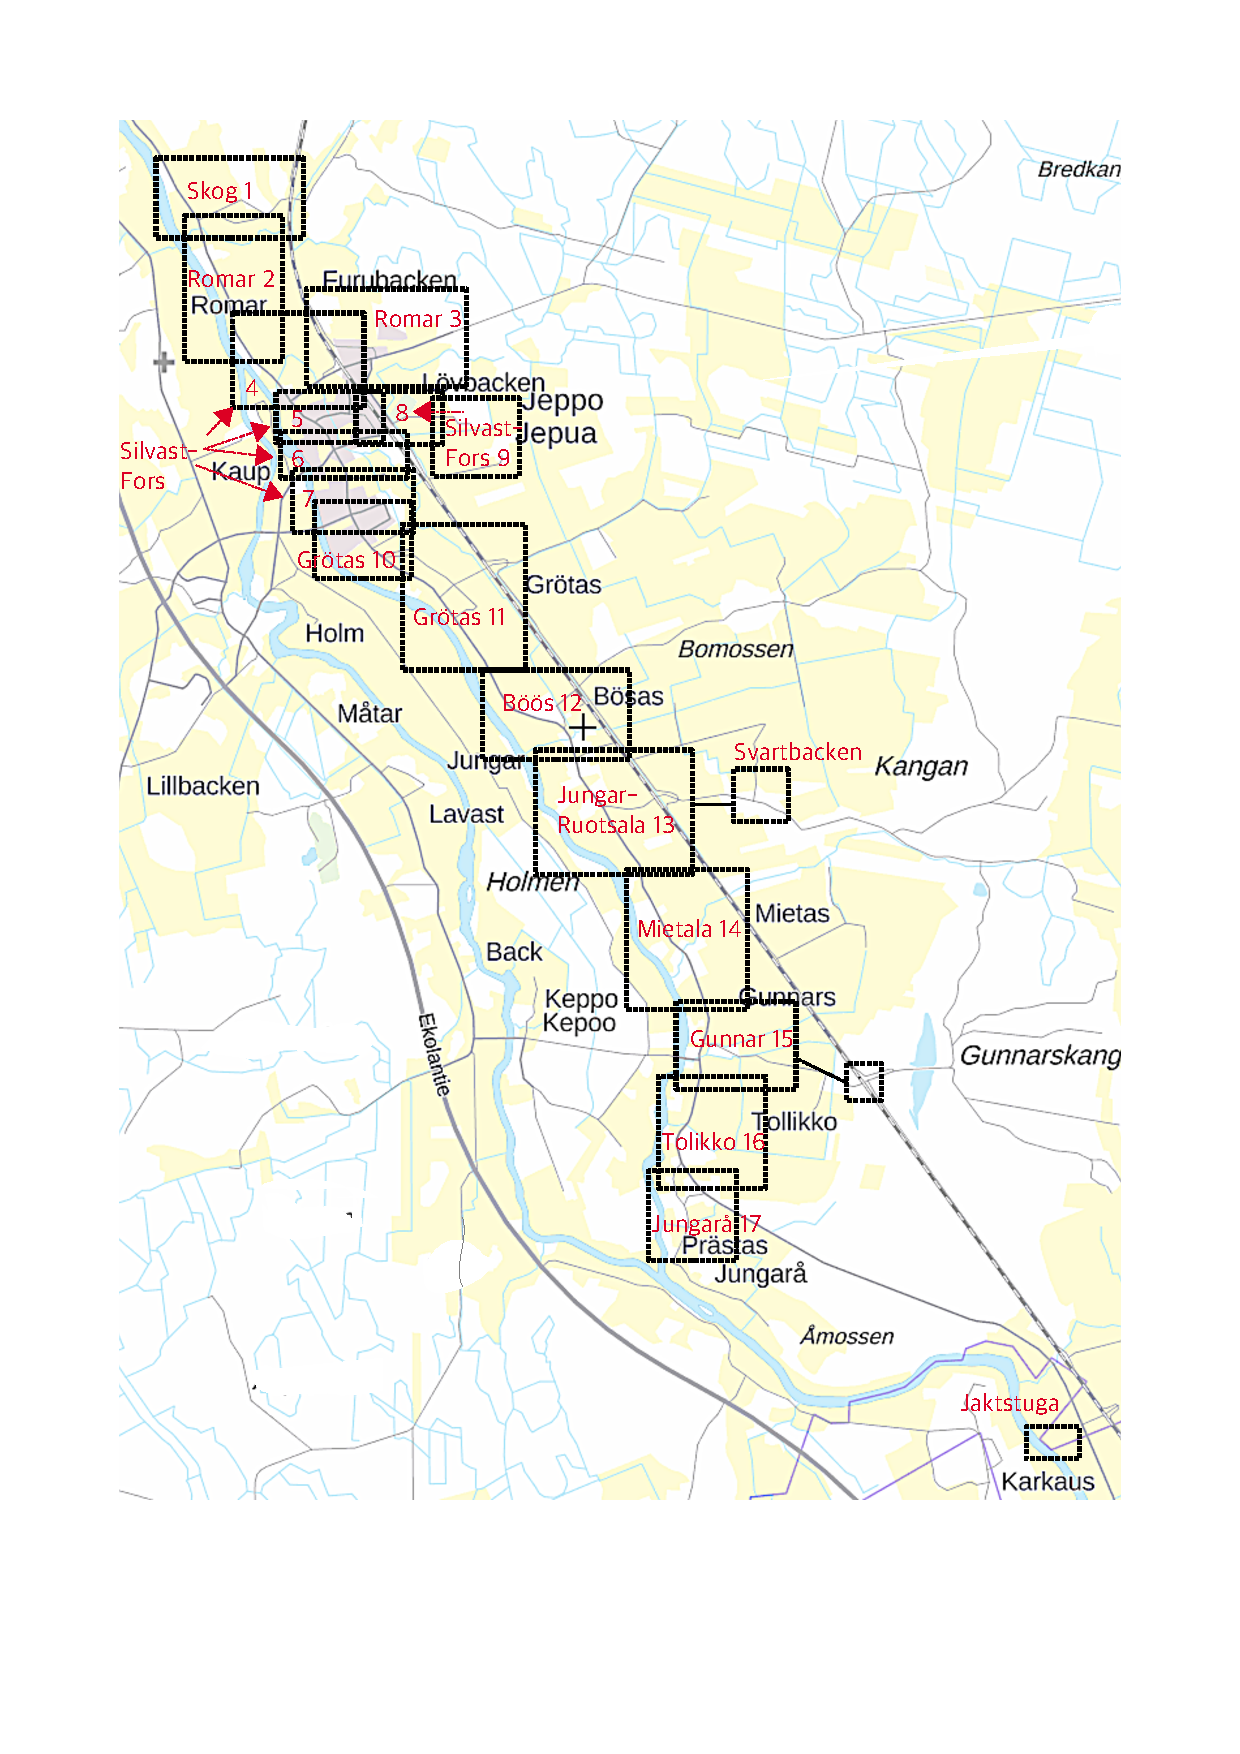
\includegraphics[width=0.95\textwidth]{kartor/Kartregister.pdf}
  \caption{Kartregistret samt kartor återfinns på sid \pageref{map:registry}}
\end{figure}
